\documentclass[11pt]{beamer}
% \usetheme{Copenhagen}
\usetheme{PaloAlto}
\usepackage[utf8]{inputenc}
\usepackage[spanish]{babel}
\usepackage{amsmath}
\usepackage{amsfonts}
\usepackage{amssymb}
\usepackage{graphicx}
\graphicspath{{figures/}}
\usepackage{ragged2e}
\usepackage{xcolor}
\usepackage{hyperref}
\hypersetup{urlcolor=blue}
\author{Carlos Espinosa}
\title{Breve historia de las computadoras}
%\setbeamercovered{transparent} 
%\setbeamertemplate{navigation symbols}{} 
\logo{
\includegraphics[width=1.4cm]{fac-logo-w}} 
\institute{Facultad de Ciencias \\ Universidad Nacional Autónoma de México} 
\date{Agosto, 2022} 
% \subject{} 

\justifying
\begin{document}

\begin{frame}
\titlepage
\end{frame}

\begin{frame}
	\tableofcontents
\end{frame}

\section{Introducción}
	\subsection{¿Qué es una computadora?}
	\begin{frame}{¿Qué es una computadora?}
		\begin{block}{Según la RAE}
			Máquina electrónica que, mediante determinados programas, permite almacenar y tratar información, y resolver problemas de diversa índole.
		\end{block}
		\begin{block}{Según la Wikipedia}
			Máquina electrónica que recibe y procesa datos para convertirlos en información conveniente y útil que posteriormente se envían a las unidades de salida.
		\end{block}
	\end{frame}
\section{Historia de las computadoras}
\subsection{Primera computadora}
\begin{frame}{¿Cuándo se creó la primera computadora?}
	Es complicado responder a la pregunta: ¿Cuál fue la primera computadora en inventarse?
	
	A lo largo de la historia, existieron diferentes máquinas que eran utilizadas para realizar cálculos:
	\begin{itemize}
		\item Ábaco: Instrumento que se remonta a las civilizaciones griega y romana
		
		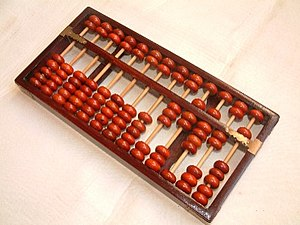
\includegraphics[scale=.25]{abaco.jpg}
		\item Pascalina: Inventada por Blaise Pascal 
		
		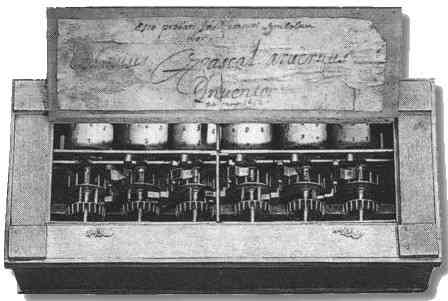
\includegraphics[scale=.15]{pascalina.jpg}
	\end{itemize}
\end{frame}
\begin{frame}{La primera computadora}
	A inicios del siglo XVII, la palabra computadora era usada para una persona que hacia cálculos. A finales del siglo XIX, la palabra cambio para usarlas en las máquinas cuya función primaria era realizar cálculos.
	
	La primera computadora mecánica (o automática) fue diseñada por Charles Babbage en 1822 llamada \textit{Difference Engine}. Era capaz de hacer cálculos de números y hacer copias físicas de los resultados.
	
	Ada Lovelace, considerada como el primer programador de computadoras ayudo a la construcción de la \textit{Difference Engine}.
	
	Babbage no pudo completar una \textit{Difference Engine} totalmente funcional por falta fondos. 
\end{frame}
\begin{frame}{La primera computadora}
	Charle Babbage propuso la primera computadora general mecánica, \textit{Analytical Engine}. Contenia una Unidad Lógica de Aritmética, control de flujo muy básico, tarjetas perforadas y memoria integrada.
	
	Igualmente, por problemas de fondos, no pudo construir una versión de esta máquina. En 1910, su hijo Henry Babbage completo una parte de esta máquina que realizaba cálculos básicos.
	
	\centering			
	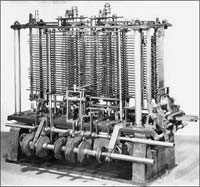
\includegraphics[scale=0.5]{analytical-engine.jpg}
\end{frame}
\begin{frame}{La primera computadora}
	La primera computadora programable fue creada por el alemán Konrad Zuse (en la sala de sus padres) entre 1936 y 1938. Es considerada la primera computadora binaria programable electro-mecánica y por lo tanto la primera computadora moderna funcional.
	
	\centering
	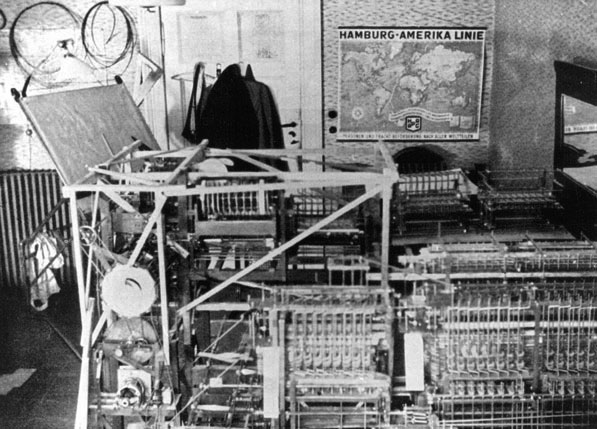
\includegraphics[scale=0.3]{z1.jpg}
\end{frame}
\subsection{Computadoras Modernas}
\begin{frame}{¿Qué se considera una computadora moderna?}
	Alan Turing propuso la maquina de Turing en 1936. Esta computadora se convirtió en la base para la teoría del computo y las computadoras. 
	
	Esta máquina fue un dispositivo que imprimía símbolos en una cinta de papel que emulaba a una persona siguiendo una seria de instrucciones lógicas. Sin estos fundamentos, no tendríamos las computadoras que usamos hoy en día.
\end{frame}
\begin{frame}{La primera computadora eléctrica programable}
	La primera computadora eléctrica programable fue la \textit{Colossus} desarrollada por Tommy Flowers en 1943. Esta máquina fue creada para ayudar a los británicos a descifrar los mensajes secretos de los alemanes.
	
	\centering
	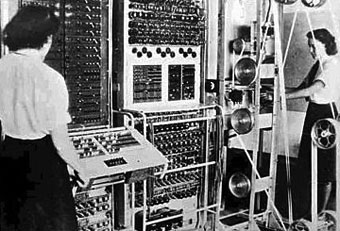
\includegraphics[scale=0.5]{colossus.jpg}
	
\end{frame}
\begin{frame}{Generaciones de las computadoras}
	A partir de esto punto, las computadoras creadas compartirán ciertas características que podemos agruparlas en lo que se llaman generaciones.
	
	Podemos distinguir, hasta ahora cinco generaciones. Cada generación compartirá, principalmente, los componentes físicos con los cuales están hechas y también se nota una progresión de los usuarios que usan las computadoras.
\end{frame}
\end{document}